\documentclass[12pt]{article}

\usepackage[margin=50pt]{geometry}
\usepackage{amsmath}
\usepackage{amssymb}
\usepackage{graphicx}
\usepackage{systeme}

\graphicspath{/images}
\geometry{footskip=0.8cm}

\title{Stochastic Decision Making}
\author{Thomas Vroom}

\begin{document}
\maketitle

%
% Chapter 1 - Probability Theory
%
\section{Probability Theory}
The set of all possible outcomes of an experiment is known as the \textbf{sample space} of the experiment and is denoted by $S$.
For example, if we are to toss a coin, the sample space is defined as $S = \{H, T\}$.
Any subset $A$ of the sample space $S$ is called an \textbf{event}.
We say that the event $A$ occurs when the outcome of the experiment lies in $A$.
The probability of an event $A$ is denoted by $P(A)$.
This function is called the \textbf{probability measure}, and has the following properties:

\begin{enumerate}
    \item $\forall A \subseteq S : 0 \leq P(A) \leq 1$
    \item $P(S) = 1$
    \item $\forall A_1, A_2, ... : P(A_i \cap A_j) = \varnothing \implies P(\cup_i A_i) = \sum_i A_i$ \hfill (Countable additivity)
    \item $P(\varnothing) = 0$
    \item $P(A^c) = 1 - P(A)$ 
    \item $P(A \cup B) = P(A) + P(B) - P(A \cap B)$
\end{enumerate}

\subsection{Conditional Probability}
The probability of event $A$, given that event $B$ has already occurred, is denoted by $P(A|B)$:
\[ P(A|B) = \frac{P(A \cap B)}{P(B)} \]

\noindent
Note that the above formula is only defined when $P(B) > 0$.
Two events $A$ and $B$ are said to be \textbf{independent} if $P(A \cap B) = P(A)P(B)$.
By the above formula, this implies that $A$ and $B$ are independent if $P(A|B) = P(A)$ (i.e. knowledge that $B$ has occurred does not affect the probability of $A$).

\noindent
\\
For a point to be in $A$, it must either be in both $A$ and $B$, or in $A$ but not in $B$:
\[ P(A) = P(A \cap B) + P(A \cap B^c) \]

\noindent
Since $P(A \cap B)$ and $P(A \cap B^c)$ are disjoint, we can write $P(A)$ as a weighted average of $P(B)$ having occurred or not:
\[ P(A) = P(A|B)P(B) + P(A|B^c)P(B^c) \]

\newpage
\noindent
Suppose that $B_1$, $B_2$, ... , $B_n$ form a partition of $S$ (i.e. exactly one of $B_i$ will occur).
Then, for any event $A$:
\[ P(A) = \sum_{i=1}^n P(A|B_i)P(B_i) \]

\noindent
This shows how we can calculate the probability of $A$ as a weighted average of $P(A|B_i)$, each weighted by the probability of $B_i$ occurring.
Suppose now that $A$ has occurred, and we are interested in determining which $B_i$ also occurred.
This is known as \textbf{Bayes' Theorem}:
\[ P(B_i | A) = \frac{P(A | B_i)P(B_i)}{\sum_{j = 1}^{n}P(A | B_j)P(B_j)} \]

\subsection{Random Variables}
It frequently occurs that in performing an experiment we are mainly interested in some functions of the outcome as opposed to the outcome itself.
A \textbf{random variable} is a function that assigns a real number to each outcome in the sample space.
For example, in the case of rolling 2 dice, we may be interested in the probability that the sum of the dice is 7.
If we define the random variable $X$ as the sum of the dice, then the question can be rephrased as finding $P(X = 7)$.

\noindent
\\
A special use of random variables is to determine if an outcome lies in an event $A$ or not:
\[ I_A = \begin{cases}
    1 & \text{if outcome lies in } A \\
    0 & \text{otherwise}
\end{cases} \]

\noindent
Here $I_A$ is known as an \textbf{indicator random variable}.

\noindent
\\
The \textbf{cumulative distribution function (CDF)} $F$ of a random variable $X$ is defined for any real number $x$ as:
\[ F(x) = P(X \leq x) \]

\noindent
In words, $F(x)$ denotes the probability that the random variable $X$ takes on a value less than or equal to $x$.
The CDF has the following properties:

\begin{enumerate}
    \item $F(x)$ is non-decreasing.
    \item $\lim_{x \to \infty} F(x) = 1$
    \item $\lim_{x \to -\infty} F(x) = 0$
    \item $P(a < X \leq b) = F(b) - F(a)$
\end{enumerate}

\subsubsection{Discrete Random Variables}
A random variable that can take on at most a countable number of possible values is said to be \textbf{discrete}.
The \textbf{probability mass function (PMF)} of a discrete random variable $X$ is defined as:
\[ p_X(x) = P(X = x) \]

\noindent
The PMF is positive for a countable number of values of $x$.
Since $X$ must take on one of these values, the sum of the PMF over all possible values must be 1:
\[ \sum_{i = 1}^{\infty} p_X(x_i) = 1 \]

\newpage
\noindent
Discrete random variables are often classified according to their PMF.
Some common examples include:

\begin{itemize}
    \item \textbf{Bernoulli Random Variable:} a single trial where $P(\text{success}) = p \in [0, 1]$ and $P(\text{failure}) = 1 - p$. $X = 1$ if the trial was successful, $X = 0$ otherwise.
    \item \textbf{Binomial Random Variable:} $n$ independent Bernoulli trials, each with probability of success $p$. $X$ is the number of successful trials:
    \[ P(X = k) = \binom{n}{k}p^k(1 - p)^{n - k}, \quad k = 0, 1, 2, ... , n \]
    \[ X \sim B(n, p) \]
    A common example is number of heads in $n$ coin flips, or the number of 6's in $n$ rolls of a die.
    \item \textbf{Geometric Random Variable:} independent Bernoulli trials (each with success probability $p$) until the first success. $X$ is the number of trials until the first success:
    \[ P(X = n) = (1 - p)^{n - 1}p, \quad n = 1, 2, 3, 4, ... \]
    \[ X \sim G(p) \]
    A common example is the number of dice rolls until a 6 comes up.
    \item \textbf{Poisson Random Variable:} the number of events occurring in a fixed time interval, given that the events occur with a known average rate $\lambda$ (i.e. we expect $\lambda$ events to occur per time unit). $X$ is the number of events in a time interval of length $t$:
    \[ P(X = k) = \frac{\lambda^k}{k!}e^{-\lambda}, \quad k = 0, 1, 2, 3, ... \]
    \[ X \sim P(\lambda t) \]
    The Poisson distribution is a limit of the binomial distribution for large $n$ and small $p$ ($\lambda = np$). 
\end{itemize}

\subsubsection{Continuous Random Variables}
A random variable that can take on an uncountable number of values is said to be \textbf{continuous}.
The \textbf{probability density function (PDF)} of a continuous random variable $X$ is defined as:
\[ P(X \in B) = \int_{B} f(x) \,dx \]

\noindent
Where $B \subseteq \mathbb{R}$.
The PDF has the following properties:

\begin{enumerate}
    \item $f$ is non-negative.
    \item $\int_{-\infty}^{\infty} f(x) \,dx = 1$
    \item $\lim_{x \to -\infty} f(x) = \lim_{x \to \infty} f(x) = 0$
    \item $P(a < X \leq b) = \int_{a}^{b} f(x) \,dx = F(b) - F(a)$ \hfill (where $B = (a, b)$)
    \item $\frac{d}{dx}F(x) = f(x)$ \hfill (PDF is the derivative of the CDF)
\end{enumerate}

\newpage
\noindent
Common examples of continuous random variables include:

\begin{itemize}
    \item \textbf{Uniform Random Variable:} $X$ is uniformly distributed on the interval $(a, b)$ if:
    \[ f(x) = \begin{cases}
        \frac{1}{b - a} & a < x < b \\
        0 & \text{otherwise}
    \end{cases}\]
    \[ X \sim U(a, b) \]
    \item \textbf{Exponential Random Variable:} how much time until the next event occurs, given that events occur at a constant rate $\lambda$. $X$ is the time until the next event:
    \[ f(x) = \begin{cases}
        \lambda e^{-\lambda x} & x \geq 0 \\
        0 & x < 0
    \end{cases} \]
    \[ X \sim Exp(\lambda) \]
    \item \textbf{Normal Random Variable:} $X$ is normally distributed with mean $\mu$ and variance $\sigma^2$ if:
    \[ f(x) = \frac{1}{\sqrt{2\pi}\sigma}e^{-\frac{(x - \mu)^2}{2\sigma^2}}, \quad -\infty < x < \infty \]
    \[ X \sim N(\mu, \sigma^2) \]
\end{itemize}

\subsubsection{Expectation}
The \textbf{expectation} of a random variable is the outcome that you get on average if you repeat the experiment many, many times.
This is not the same as the most likely outcome.
The expected value of a random variable $X$ is calculated as a weighted average of all the possible values that $X$ can take on:
\[ E(X) = \begin{cases}
    \displaystyle \sum_{x:p(x)>0} xp(x) & \text{if } X \text{ is discrete} \\
    \displaystyle \int_{-\infty}^{\infty} xf(x) \,dx & \text{if } X \text{ is continuous}
\end{cases} \]

\noindent
Let $I_A$ be an indicator random variable for an event $A$.
Then $E(I_A) = P(A)$.

\begin{table}[h]
    \centering
    \begin{tabular}{c|c}
    $X$                       & $E(X)$               \\ \hline
    $X \sim Bernoulli(p)$     & $p$                  \\
    $X \sim B(n, p)$          & $np$                 \\
    $X \sim G(p)$             & $\frac{1}{p}$        \\
    $X \sim P(\lambda)$       & $\lambda$            \\
    $X \sim U(a, b)$          & $\frac{1}{2}(a + b)$ \\
    $X \sim Exp(\lambda)$     & $\frac{1}{\lambda}$  \\
    $X \sim N(\mu, \sigma^2)$ & $\mu$               
    \end{tabular}
    \caption{The expected value of random variables with common distributions.}
\end{table}

\newpage
\noindent
To calculate the expected value of a function, we can use the same formula as shown above:
\[ E(g(X)) = \begin{cases}
    \displaystyle \sum_{x:p(x)>0} g(x)p(x) & \text{if } X \text{ is discrete} \\
    \displaystyle \int_{-\infty}^{\infty} g(x)f(x) \,dx & \text{if } X \text{ is continuous}
\end{cases} \]

\noindent
Some useful cases include:
\begin{align*}
    E(aX + b) & = aE(X) + b \\
    E(X^n) & = \int_{-\infty}^{\infty} x^n f(x) \,dx \\
    E(I_A) & = P(A)
\end{align*}

\noindent
Similar to the expectation, the \textbf{variance} of a random variable is another quantity of interest.
The variance of a random variable measures the distance from the expected value:
\[ Var(X) = E((X - E(X))^2) = E(X^2) - E^2(X) \]

\begin{table}[h]
    \centering
    \begin{tabular}{c|c}
    $X$                       & $Var(X)$               \\ \hline
    $X \sim Bernoulli(p)$     & $p(1 - p)$                  \\
    $X \sim B(n, p)$          & $np(1 - p)$                 \\
    $X \sim G(p)$             & $\frac{1}{p^2}$        \\
    $X \sim P(\lambda)$       & $\lambda$            \\
    $X \sim U(a, b)$          & $\frac{1}{12}(b - a)^2$ \\
    $X \sim Exp(\lambda)$     & $\frac{1}{\lambda^2}$  \\
    $X \sim N(\mu, \sigma^2)$ & $\sigma^2$               
    \end{tabular}
    \caption{The variance of random variables with common distributions.}
\end{table}

\subsubsection{Joint Random Variables}
We are often interested in probability statements concerning two or more random variables.
The \textbf{joint probability mass function (PMF)} of two \textbf{discrete} random variables $X$ and $Y$ is defined as:
\[ p(x, y) = P(X = x, Y = y) \]

\noindent
The \textbf{marginal PMF} of $X$ and $Y$ are defined as:
\begin{alignat*}{2}
    P(X = x) &= p_X(x) & &= \sum_{y:p(x, y) > 0} p(x, y) \\
    P(Y = y) &= p_Y(y) & &= \sum_{x:p(x, y) > 0} p(x, y)
\end{alignat*}

\noindent
We say that $X$ and $Y$ are \textbf{jointly continuous} if there exists a function $f(x, y)$ such that:
\[ P(X \in A, Y \in B) = \int_A \int_B f(x, y) \,dxdy \]

\newpage
\noindent
The \textbf{marginal PDF} of $X$ and $Y$ are defined as:
\begin{alignat*}{2}
    f_X(x) &= \int_{-\infty}^{\infty} f(x, y) \,dy \\
    f_Y(y) &= \int_{-\infty}^{\infty} f(x, y) \,dx
\end{alignat*}

\noindent
Two random variables $X$ and $Y$ are said to be \textbf{independent} if:

\begin{enumerate}
    \item $p(x, y) = p_X(x) \cdot p_Y(y)$ (if $X$ and $Y$ are discrete)
    \item $f(x, y) = f_X(x) \cdot f_Y(y)$ (if $X$ and $Y$ are continuous)
\end{enumerate}

\noindent
The expected value of a function of two or more random variables is calculated in the same way as for a single random variable:
\[ E(a_1X_1 + a_2X_2 + ... + a_nX_n) = a_1E(X_1) + a_2E(X_2) + ... + a_nE(X_n) \]

\subsection{Conditional Probability}
One of the most useful concepts in probability theory is that of conditional probability.
The reason is twofold: First, in practice, we are often interested in calculating probabilities and expectations when some partial information is available; hence, the desired probabilities and expectations are conditional ones. 
Secondly, in calculating a desired probability or expectation it is often extremely useful to first \textit{condition} on some appropriate random variable.
For discrete random variables, the conditional PMF of $X$ given $Y = y$ is defined as:
\[ p_{X|Y}(x|y) = P(X = x | Y = y) = \frac{P(X = x, Y = y)}{P(Y = y)} = \frac{p(x, y)}{p_Y(y)} \]

\noindent
For continuous random variables, the conditional PDF of $X$ given $Y = y$ is defined as:
\[ f_{X | Y}(x | y) = \frac{f(x, y)}{f_Y(y)} \]

\noindent
Note that in both cases, the conditional PMF or PDF is only defined when $P(Y = y) > 0$.
In terms of conditional probabilities, $X$ and $Y$ are independent if:

\begin{enumerate}
    \item $p(x, y) = p_X(x) \cdot p_Y(y) \implies p_{X|Y}(x|y) = p_X(x) \ \forall x \forall y$ (if $X$ and $Y$ are discrete)
    \item $f(x, y) = f_X(x) \cdot f_Y(y) \implies f_{X|Y}(x|y) = f(x) \ \forall Y$ (if $X$ and $Y$ are continuous)
\end{enumerate}

\subsubsection{Conditional Expectation}
Let us denote by $E(X|Y)$ a function of the variable $Y$ whose value at $Y = y$ is $E(X | Y = y)$.
Note that $E(X|Y)$ is itself a random variable.
In important property of conditional expectation is that for all random variables $X$ and $Y$:
\[ E(X) = E(E(X|Y)) = \begin{cases}
    \displaystyle \sum_{y : p_Y(y) > 0} E(X|Y = y)p_Y(y) & \text{if } Y \text{ is discrete} \\
    \displaystyle \int_{-\infty}^{\infty} E(X|Y = y)f_Y(y) \,dy & \text{if } Y \text{ is continuous}
\end{cases} \]

\newpage
\noindent
The variance of a random variable can be calculated using the law of total variance:
\[ Var(X) = E(Var(X|Y)) + Var(E(X|Y)) \]
\[ Var(X|Y = y) = E(X^2|Y = y) - E^2(X|Y = y) \]

\noindent
Furthermore:
\[ E(Var(X|Y)) = \begin{cases}
    \displaystyle \sum_{y : p_Y(y) > 0} Var(X|Y = y)p_Y(y) & \text{if } Y \text{ is discrete} \\
    \displaystyle \int_{-\infty}^{\infty} Var(X|Y = y)f_Y(y) \,dy & \text{if } Y \text{ is continuous}
\end{cases} \]
\[ Var(E(X|Y)) = \begin{cases}
    \displaystyle \sum_{y : p_Y(y) > 0} (E(X|Y = y) - E(X))^2p_Y(y) & \text{if } Y \text{ is discrete} \\
    \displaystyle \int_{-\infty}^{\infty} (E(X|Y = y) - E(X))^2f_Y(y) \,dy & \text{if } Y \text{ is continuous}
\end{cases} \]

\subsubsection{Probabilities by Conditioning}
For any event $A$ we can define the indicator random variable $I_A$, which is 1 if $A$ occurs and 0 otherwise.
We have $E(I_A) = P(A)$, as well as $E(I_A|Y = y) = P(A|Y = y)$.
By combining this with the above formulas for conditional expectation, we can calculate probabilities by conditioning:
\[ P(A) = \begin{cases}
    \displaystyle \sum_{y : p_Y(y) > 0} P(A | Y = y)p_Y(y) & \text{if } Y \text{ is discrete} \\
    \displaystyle \int_{-\infty}^{\infty} P(A | Y = y)f_Y(y) \,dy & \text{if } Y \text{ is continuous}
\end{cases} \]

\noindent
A collection of random variables $X = X_1, X_2, X_3, ... , X_n$ is called \textbf{exchangeable} if the joint probability mass / density function remains unchanged if we change the order of the random variables.
If $X$ is an independent and identically distributed (IID) sample, then $X$ is exchangeable.
However, the converse does not hold true.
An important property of exchangeable random variables is that they share the same probability distribution.

%
% Chapter 2 - Markov Chains
%
\newpage
\section{Markov Chains}
A Markov chain is a stochastic process where the conditional distribution of future states depends only on the current state, and not on the sequence of events that preceded it.
The value $P_{ij}$ denotes the probability of transitioning from state $i$ to state $j$.
This value has the following properties:
\begin{align*}
    \displaystyle P_{ij} \geq 0 && \sum_{j = 0}^\infty P_{ij} = 1
\end{align*}

\noindent
The \textbf{transition matrix} $P$ is defined as:
\[ P = \begin{bmatrix}
    P_{00} & P_{01} & P_{02} & ... \\
    P_{10} & P_{11} & P_{12} & ... \\
    P_{20} & P_{21} & P_{22} & ... \\
    \vdots & \vdots & \vdots & \ddots
\end{bmatrix} \]

\subsection{State Classification}
A state $s_i$ can be reached from state $s_j$ if there exists a sequence of states $s_{k_1}, s_{k_2}, ... , s_{k_n}$ such that $P_{jk_1}P_{k_1k_2}...P_{k_ni} > 0$.
A state is \textbf{transient} if there is a non-zero probability that the chain will never return to that state.
A state is \textbf{recurrent} if it is visited infinitely often.
A process starting in a recurrent state will by definition return to that state.
A state is \textbf{absorbing} if it is recurrent and there is no way to leave that state:

\begin{figure}[h]
    \centering
    \begin{minipage}{.5\textwidth}
      \centering
      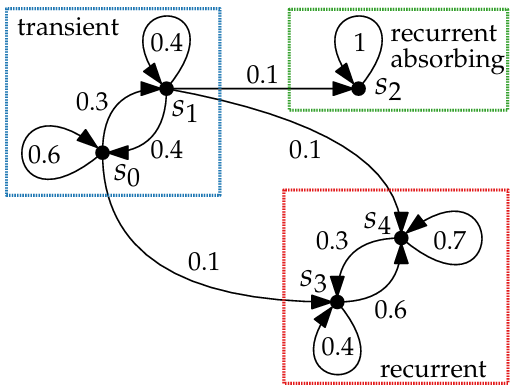
\includegraphics[scale=0.6]{images/markovchain.PNG}
    \end{minipage}%
    \begin{minipage}{.5\textwidth}
      \centering
      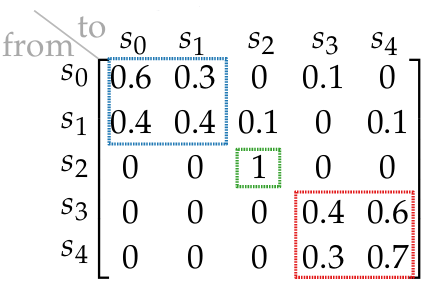
\includegraphics[scale=0.7]{images/transitionmatrix.PNG}
    \end{minipage}
\end{figure}

\noindent
Let $P_{ij}^n$ be the probability of transitioning from state $i$ to state $j$ in $n$ steps.
This is called the \textbf{$n$-step transition probability}.
The $n$-step transition matrix can be calculated by multiplying the transition matrix $P$ by itself $n$ times.
We can use the $n$-step transition probability to give a more formal definition of transient and recurrent states:
\[ \sum_{n = 1}^\infty P_{ii}^n \begin{cases}
    < \infty & \text{state } i \text{ is transient} \\
    = \infty & \text{state } i \text{ is recurrent}
\end{cases} \]

\noindent
Note that $P_{ij}^n$ is conditioned on the initial state $i$.
The unconditional probability of transitioning to state $j$ in $n$ steps is given by:
\[ P(X_n = j) = \sum_{i = 0}^\infty P_{ij}^n \alpha_i \]

\noindent
Where $\alpha_i$ is the probability of starting in state $i$.

\newpage
\noindent
Let $\mathbb{A} \subseteq S$ be a set of states, and suppose we are interested in the probability that the Markov chain ever enters any of the states in $\mathbb{A}$ by time $m$.
That is, for a given state $i \notin \mathbb{A}$ , we are interested in determining:
\[ P(X_k \in \mathbb{A} \text{ for some } k = 1, ... , m | X_0 = i) \]

\noindent
To find this probability, we introduce a new absorbing state $A$, that replaces all states in $\mathbb{A}$.
The probability of entering any state in $\mathbb{A}$ is the same as the probability of entering state $A$: $P_{iA}^m$

\subsection{Communication and Classes}
State $s_j$ is said to be \textbf{accessible} from state $s_i$ if $P_{ij}^n > 0$ for some $n \geq 0$.
Two states $s_i$ and $s_j$ are said to \textbf{communicate} if $s_j$ is accessible from $s_i$ and $s_i$ is accessible from $s_j$: $s_i \leftrightarrow s_j$.
The relation of communication has the following properties:

\begin{enumerate}
    \item All states communicate with themselves: $s_i \leftrightarrow s_i$.
    \item If state $s_i$ communicates with state $s_j$, then $s_j$ communicates with $s_i$: $s_i \leftrightarrow s_j \implies s_j \leftrightarrow s_i$.
    \item If state $s_i$ communicates with state $s_j$ and state $s_j$ communicates with state $s_k$, then state $s_i$ communicates with state $s_k$: $s_i \leftrightarrow s_j \text{ and } s_j \leftrightarrow s_k \implies s_i \leftrightarrow s_k$.
\end{enumerate}

\noindent
Two states $s_i$ and $s_j$ are said to be in the same \textbf{class} if $s_i \leftrightarrow s_j$.
If a state is transient or recurrent, then any state in the same class is also transient or recurrent.
A Markov chain is said to be:

\begin{itemize}
    \item \textbf{Irreducible} if all states are in the same class.
    \item \textbf{Unichained} if it has, beside transient states, only one class of recurrent states.
\end{itemize}

\noindent
A state $s_i$ is said to be \textbf{periodic} if the chain can only return to $s_i$ in multiples of some integer $d > 1$.
In other words, $d$ is the greatest common divisor such that $P_{ii}^n = 0$ if $n$ is divisible by $d$.
If $d = 1$, then the state is said to be \textbf{aperiodic}.
Periodicity is a class property, meaning that if one state in a class is periodic with period $d$, then all states in that class are periodic with period $d$.
Recurrent, aperiodic states are called \textbf{ergodic}.

\subsection{Limiting Probabilities}
Each Markov chain has a unique vector $\pi$, where $\pi_i$ is the fraction of time spend in state $s_i$.
This is known as the \textbf{steady-state probability vector}.
If the Markov chain is irreducible, then $\pi$ has the following properties:

\begin{itemize}
    \item $\displaystyle \sum_{i} \pi_i = 1$ \hfill (the sum of all probabilities is 1)
    \item $\pi P = \pi$ \hfill (the probabilities are independent of the starting state)
\end{itemize}

\noindent
Let $Q$ be the $\infty$-step transition matrix, with $\displaystyle Q_{ij} = \lim_{t \rightarrow \infty} P_{ij}^t$.
If the Markov chain is aperiodic, each row $i$ of $Q$ is the steady-state probability vector $\pi$ for starting in state $i$.
If the Markov chain is also irreducible, then each row of $Q$ is the same steady-state probability vector $\pi$: $Q_{ij} = \pi_j$ (the limiting probability that the process will be in state $j$).

\newpage
\noindent
We can find the steady-state probabilities by solving the equation $\pi = \pi P$, for example:
\begin{align*}
    (\pi_0, \pi_1, \pi_2) = (\pi_0, \pi_1, \pi_2)\begin{bmatrix}
        0 & 1 & 0 \\
        \frac{1}{2} & 0 & \frac{1}{2} \\
        \frac{1}{2} & 0 & \frac{1}{2}
    \end{bmatrix} && \systeme{
        \pi_0 = \frac{1}{2}\pi_1 + \frac{1}{2}\pi_2,
        \pi_1 = \pi_0,
        \pi_2 = \frac{1}{2}\pi_1 + \frac{1}{2}\pi_2,
        1 = \pi_0 + \pi_1 + \pi_2
    }
\end{align*}

\noindent
Solving this system of equations, we find $\pi = \left( \frac{1}{3}, \frac{1}{3}, \frac{1}{3} \right)$.

\noindent
\\
The proportion of time spent in a state $s_i$ is given by the steady-state probability $\pi_i$.
The inverse of this value is known as the \textbf{mean recurrence time}, the average number of transitions required to return to state $s_i$:
\[ m_{ii} = \frac{1}{\pi_i} \]

\noindent
To find the average number of visits to a transient state $s_j$, we can use the following formula:
\[ S = (I - P_T)^{-1} \]

\noindent
Where $S_{ij}$ is the expected number of visits to state $s_j$ starting from state $s_i$, and $P_T$ is the transient part of the transition matrix $P$ (with all recurrent states cut out).

\noindent
\\
Let $f_{ij}$ be the probability of transitioning from transient state $s_i$ to transient state $s_j$ without visiting any recurrent states.
This is calculated as:
\begin{align*}
    f_{ij} = \frac{s_{ij} - \delta_{ij}}{s_{jj}} && \delta_{ij} = \begin{cases}
        1 & i = j \\
        0 & i \neq j
    \end{cases}
\end{align*}

\subsection{Time Reversible Markov Chains}
Consider an ergodic Markov chain that is \textbf{stationary} (i.e. the Markov chain has been in operation for a long time) with transition probabilities $P_{ij}$ and stationary probabilities $\pi_i$.
Starting at some time $t$, we trace the chain backwards in time: $X_t, X_{t - 1}, X_{t - 2}, ...$.
This sequence of states is itself a Markov chain with transition probabilities:
\[ Q_{ij} = \frac{\pi_j P_{ji}}{\pi_i} \]

\noindent
If $Q_{ij} = P_{ij}$ for all $i, j$, then the Markov chain is said to be \textbf{time reversible}.
This property is equivalent to stating that a Markov chain is time reversible if the rate at which the process goes from $i$ to $j$ is equal to the rate at which the process goes from $j$ to $i$, for all $i, j$:
\[ \pi_i P_{ij} = \pi_j P_{ji} \]

\noindent
A Markov chain can be visualized as a directed graph, where each vertex corresponds to a state in the chain, and each edge from $i$ to $j$ represents a transition from state $i$ to state $j$ (written down as $i \rightarrow j$).
A \textbf{circuit} in a graph is a walk that starts and ends at the same vertex, while a \textbf{cycle} is a circuit that does not visit any vertex more than once.
A $k$-cycle is a cycle that consists of $k$ edges.
An irreducible Markov chain with only 1- and 2-cycles is always time reversible.

\newpage
\noindent
An ergodic Markov chain for which $P_{ij} = 0$ whenever $P_{ji} = 0$ is time reversible if and only if starting in state $i$, any path back to $i$ has the same probability as the reverse path:
\[ P_{i,i_1} P_{i_1,i_2} ... P_{i_k,i} = P_{i,i_k} P_{i_k,i_{k-1}} ... P_{i_1,i} \]

\noindent
An important example is a Markov chain corresponding to a random walk on a connected, undirected graph with edge weights:

\begin{figure}[h]
    \centering
    
\includegraphics[scale=0.6]{images/markovchain2.PNG}
\end{figure}

\noindent
This graph has weights $w_{ij} = w_{ji}$ for each edge $ij$.
If there is no edge between $i$ and $j$, then $w_{ij} = 0$.
The transition probability from state $i$ to state $j$ is given by:
\[ P_{ij} = \frac{w_{ij}}{\displaystyle \sum_{k = 1}^{n} w_{ik}} \]

\noindent
The Markov chain is irreducible, since the graph is strongly connected, and it is also time reversible.
For this kind of Markov chain, we can calculate the steady-state probability $\pi_i$ as:
\[ \pi_i = \frac{\displaystyle \sum_{k = 1}^n w_{ij}}{\displaystyle \sum_{i = 1}^n \sum_{k = 1}^n w_{ik}} \]

\noindent
In this example we have $\displaystyle \sum_{k = 1}^n w_{ij} = 9, 13, 10, 6$ if $i$ is $1, 2, 3, 4$ respectively.
This means that the steady-state probabilities are given as $\pi = \frac{1}{38}(9, 13, 10, 6)$, which we now know without having to solve $\pi P = \pi$.

%
% Chapter 3 - Markov Decision Processes
%
\newpage
\section{Markov Decision Processes}
\subsection{Definitions}
A \textbf{Markov Decision Process (MDP)} is a decision process where a single decision maker tries to maximize a reward in a stochastic environment.
An MDP $\Gamma$ is defined by a tuple $(S, A, P, r)$:

\begin{itemize}
    \item A finite set of states $S = \{s_0, s_1, ... , s\}$.
    \item For each state $s \in S$, a finite set of actions $A_s = \{a_1, a_2, ... , m(s)\}$, where $m(s)$ is the number of actions in state $s$. We also define $A$ as the set of all actions available in the MDP.
    \item For each state $s \in S$ and action $a \in A_s$, a \textbf{transition probability}: 
    \[ P(s^\prime | s, a) = P(s_{n + 1} = s^\prime | s_n = s, a_n = a) \]
    \item For each state $s \in S$ and action $a \in A_s$, a payoff $r(s, a)$.
\end{itemize}

\noindent
Note that $a_s$ denotes the action taken in state $s$, while $a_n$ denotes the action taken at time $n$.
Take the following MDP $\Gamma$ as an example:

\begin{figure}[h]
    \centering
    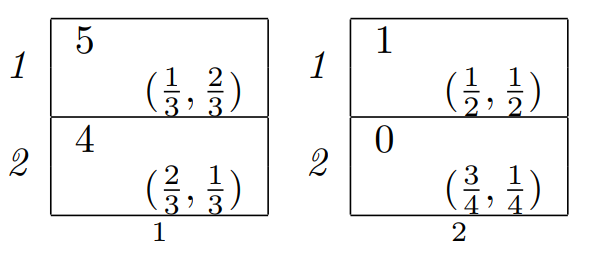
\includegraphics[scale=0.5]{images/mdp_example.PNG}
\end{figure}

\noindent
$\Gamma$ has two states: $1$ and $2$, represented by the columns.
In both states the player has two actions, written to the left of the corresponding cell.
The payoff for each action is written in the top-left of the cell, while the transition probability is written in the bottom-right.
If in this example the player plays action $1$ in state $1$, then they receive a payoff of $5$.
With probability $\frac{1}{3}$ the state transitions to state $1$ again, while with probability $\frac{2}{3}$ the state transitions to state $2$.

\noindent
\\
If a player has more than one action available in a state, they are allowed to randomize over their available actions in $A_s$.
This is called a \textbf{mixed action}, and is denoted by $f(s)$, where $f(s)$ is a probability distribution over $A_s$.
The set of all mixed actions in a state is denoted by $F_s$, and the set of all mixed actions in the MDP is denoted by $F$.
In this definition, any pure action is also a mixed action.

\subsubsection{Strategies}
A \textit{play} or \textit{realization} of an MDP is a sequence of states and actions $s_0, a_0, s_1, a_1, ...$, where each $a_n \in A_{s_n}$ represents the (mixed) action taken at stage $n$, whereas each $s_n$ represents the state at stage $n$.
A finite sequence $s_0, a_0, s_1, a_1, ... , s_{n-1}, a_{n - 1}, s_n = h_n$ is called the \textbf{history} until stage $n$.
The set of all histories is denoted by $H$.
A \textbf{strategy} $\sigma$ is a function that assigns to each history a mixed action:
\[ \sigma: H \rightarrow F \]

\noindent
Note that a strategy is also called a \textbf{control} or a \textbf{policy}.

\newpage
\noindent
A strategy is \textbf{stationary} if it only depends on the current state:
\[ f: S \rightarrow F \]

\noindent
A stationary strategy prescribes to play the same mixed action each time it visits a state, independent of the history.
Let $f(s, a)$ denote the probability that the mixed action $f(s)$ selects action $a$ in state $s$.
We can use this to define a stationary strategy as:
\[ f = (f(0), f(1), ... , f(s)) \]

\noindent
A strategy is called \textbf{pure} if it always prescribes a pure action:
\[ \sigma: H \rightarrow A \]

\noindent
As a result, a strategy that is both stationary and pure can be described as:
\[ f: S \rightarrow A \]

\noindent
A useful property of a stationary strategy is that it determines a stochastic matrix with the following entries:
\[ P_f(s, s^\prime) = p(s^\prime | s) = \sum_{a = 1}^{m(s)} p(s^\prime | s, a) \cdot f(s, a) \]

\noindent
Looking back at the example MDP $\Gamma$, we find:
\begin{align*}
    p_f(1 | 1) & = p(1 | 1, 1) \cdot f(1, 1) + p(1 | 1, 2) \cdot f(1, 2) \\
    & = \frac{1}{3} \cdot \frac{1}{4} \cdot \frac{2}{3} \cdot \frac{3}{4} \\
    & = \frac{7}{12} \\
    p_f(2 | 1) & = p(2 | 1, 1) \cdot f(1, 1) + p(2 | 1, 2) \cdot f(1, 2) \\
    & = \frac{2}{3} \cdot \frac{1}{4} \cdot \frac{1}{3} \cdot \frac{3}{4} \\
    & = \frac{5}{12} \\
    p_f(1 | 2) & = p(1 | 2, 1) \cdot f(2, 1) + p(1 | 2, 2) \cdot f(2, 2) \\
    & = \frac{1}{2} \cdot 1 \cdot \frac{3}{4} \cdot 0 \\
    & = \frac{1}{2} \\
    p_f(2 | 2) & = p(2 | 2, 1) \cdot f(2, 1) + p(2 | 2, 2) \cdot f(2, 2) \\
    & = \frac{1}{2} \cdot 1 \cdot \frac{1}{4} \cdot 0 \\
    & = \frac{1}{2}
\end{align*}
\[ P_f = \begin{bmatrix}
    \frac{7}{12} & \frac{5}{12} \\
    \frac{1}{2} & \frac{1}{2}
\end{bmatrix} \]

\noindent
The (fixed) probabilities of the stationary strategy $f$ induce a stationary Markov chain.

\newpage
\subsubsection{Payoffs}
We distinguish between two types of payoffs in an MDP:

\begin{enumerate}
    \item The payoffs corresponding to the state-action pairs (listed in the cells of the MDP), denoted by $r(s, a)$.
    \item The \textbf{stage payoffs}, denoted by $R_n(s_0, f)$.
\end{enumerate}

\noindent
The stage payoff $R_n(s_0, f)$ is the expected payoff at stage $n$ when the MDP starts in state $s_0$ and the player follows the strategy $f$.
Note that $R_n(s_0, f)$ is a random variable whose value depends on the state visited at stage $n$ and the prescribed (mixed) action there.
To calculate the expected value of a payoff, we can use the following formula:
\[ r(s, f) = \sum_{a = 1}^{m(s)} r(s, a) \cdot f(s, a) \]

\noindent
Using a strategy $f$ in an MDP $\Gamma$ generates an infinite stream of stage payoffs that need to be evaluated.
The most common ways to do this are:

\begin{enumerate}
    \item Discounting the stage payoffs using a discount factor $\beta \in [0, 1)$. This results in the \textbf{$\beta$-discounted MDP $\Gamma_\beta$}.
    \item Taking the sum of the stage payoffs. This results in the \textbf{total reward MDP $\Gamma_\tau$}, and is only possible if the sum of the stage payoffs is finite.
    \item Taking the average of the stage payoffs. This results in the \textbf{average reward MDP $\Gamma_\alpha$}. 
\end{enumerate}

\noindent
The resulting number is called the \textbf{reward} of the strategy $f$ in $\Gamma$, which may depend on the initial state $s_0$.

\subsection{Optimal Strategies}
\subsubsection{Discounted MDPs}
In $\Gamma_\beta$, the $\beta$-discounted reward of strategy $f$, starting in state $s_0$, is given by:
\[ \gamma_\beta(s_0, f) = \sum_{n = 0}^\infty \beta^n \cdot E(R_n(s_0, f)) \]

\noindent
The discounted reward is the sum of all the discounted stage payoffs.
As long as $\beta < 1$, this sum is finite.
If we consider the reward for all initial states simultaneously, we get:
\[ \gamma_\beta(f) = \sum_{n = 0}^\infty \beta^n \cdot E(R_n(f)) = (I - \beta \cdot P_f)^{-1} r(f) \]

\noindent
For any stationary strategy $f$, the matrix $P_f$ and the vector $r(f)$ can easily be found.
The easiest way to calculate $\gamma_\beta(f)$ is to then solve the following system of linear equations:
\[ (I - \beta \cdot P_f) \gamma_\beta(f) = r(f) \]

\newpage
\noindent
The next step of the analysis is to find, if possible, a strategy that maximizes the reward.
Let $\Gamma_\beta$ be a $\beta$-discounted MDP.
There exists a pure stationary strategy $f^*$ that maximizes $\gamma_\beta(f)$ in $\Gamma_\beta$.
This maximum, called $\upsilon_\beta$, is the (state-dependent) \textbf{$\beta$-discounted value} of $\Gamma_\beta$, and $f^*$ is called a \textbf{($\beta$-discounted) optimal strategy}.
Note that it is possible for a discounted MDP to have more than one optimal strategy.
In such a case, all optimal strategies have the same value vector $\upsilon_\beta$.

\subsubsection{Terminating MDPs}
A decision problem is called \textbf{terminating} if eventually the process terminates, independent of the player's strategy.
In other words, there exist one or more states where with positive probability the process terminates.
This decision problem is not an MDP, since the process does not continue indefinitely.
However, we can transform this kind of decision problem into an MDP by adding an artificial absorbing state $0$ that has only one action with a payoff of $0$.
The resulting MDP is called a \textbf{terminating MDP}.

\noindent
\\
If $\Gamma$ is a terminating MDP, then the sum of the stage payoffs in $\Gamma$ is finite.
This sum of the stage payoffs is called the \textbf{total reward}, and can act as a measure of quality for a strategy.
Terminating MDPs are often used to find optimal strategies in situations where the objective is to reach a certain state as quick as possible.

\noindent
\\
For every stationary strategy $f$ in a total reward MDP $\Gamma_\tau$, we can calculate its total reward $\gamma_\tau(f)$ similarly to calculating the discounted reward:
\[ \gamma_\tau(f) = \sum_{n = 0}^\infty P_T^n(f) \cdot r(f) = (I - P_T(f))^{-1} r(f) \]

\noindent
Where $P_T(f)$ is the transient part of the transition matrix $P$ of the Markov chain induced by $f$.
Just like a discounted MDP, the reward for the terminating MDP can also be calculated by solving the following system of linear equations:
\[ (I - P_T(f)) \cdot \gamma_\tau(f) = r(f) \]

\noindent
Let $\Gamma_\tau$ be a terminating MDP.
There exists a pure stationary strategy $f^*$ that maximizes $\gamma_\tau(f)$ in $\Gamma_\tau$.
This maximum, called $\upsilon_\tau$, is the (state-dependent) \textbf{value} of $\Gamma_\tau$, and $f^*$ is called an \textbf{optimal strategy}.

\subsubsection{Average Reward MDPs}
The MDP $\Gamma_\alpha$, called the \textbf{average reward MDP}, results from taking the average of the stage payoffs.
For a stationary strategy $f$ in $\Gamma_\alpha$, the average reward $\gamma_\alpha(f)$ is given by:
\[ \gamma_\alpha(f) = \lim_{T \rightarrow \infty} \frac{1}{T + 1} \sum_{n = 0}^T P^n(f) \cdot r(f) \]

\noindent
Note that the average reward is the limit of the average of the stage payoffs as the number of stages approaches infinity.
This has some implications for the calculation of the average reward.
For example, if a strategy has only a $0.1\%$ chance of reaching an absorbing state, then the average reward will be $0$, even though it might take thousands of stages to reach the absorbing state.

\newpage
\noindent
We assume that if the player uses a pure strategy $f$, then the resulting Markov chain $P(f)$ has exactly one recurrent class.
An MDP with this property is called \textbf{unichained}.
For any unichained Markov chain, we can calculate the Cesaro-limit of the transition matrix $P(f)$:
\[ Q(f) = \lim_{t \rightarrow \infty} \frac{1}{T + 1} \sum_{n = 0}^T P^n(f) \]

\noindent
Using this, we can also calculate the average reward as follows:
\[ \gamma_\alpha(f) = Q(f) \cdot r(f) \]

\noindent
It can be shown that for any unichained MDP and for any stationary strategy the matrix $Q(f)$ has identical rows, and that the entries of each row correspond to the limiting probabilities of the induced Markov chain.
This means that the average reward of a stationary strategy in a unichained MDP is state-independent.

\noindent
\\
Let $\Gamma_\alpha$ be a unichained MDP with a finite state space $S = \{ 1, 2, ... , s_z \}$ and let $f$ be a stationary strategy.
Then $f$ induces a unichained Markov Chain with limiting probabilities $\pi(f)$ and:
\[ \gamma_\alpha(f) = \lim_{T \rightarrow \infty} \frac{1}{T + 1} \sum_{n = 0}^T E(R_n(f)) = \sum_{s = 1}^{s_z} r(s, f) \cdot \pi_s(f) \]

\noindent
Let $\Gamma$ be an MDP with corresponding $\beta$-discounted MDPs $\Gamma_\beta$ for all $\beta \in [0, 1)$ and corresponding average reward MDP $\Gamma_\alpha$.
There exists a $\beta^0 \in [0, 1)$ and a pure stationary strategy $f^*$ such that for all $\beta \in [\beta^0, 1)$:
\begin{align*}
    \gamma_\beta(f^*) &= \max_{f \in F_D} \gamma_\beta(f) \\ \gamma_\alpha(f^*) &= \max_{f \in F_D} \gamma_\alpha(f)
\end{align*}

\noindent
Where $F_D$ is the set of all pure strategies in $\Gamma$.
If $f^*$ is optimal in $\Gamma_\beta$ for all $\beta \in [\beta^0, 1)$, then $f^*$ is called \textbf{uniformly optimal}, and is also optimal in $\Gamma_\alpha$.
Furthermore, if $\Gamma$ is unichained, then this value is state-independent.
The state-independent value for an unichained MDP that has a pure stationary optimal strategy $f^*$ is equal to:
\[ \upsilon_\alpha = \gamma_\alpha(f^*) = \sum_{s = 1}^{s_z} r(s, f^*) \cdot \pi_s(f^*) \]

\subsection{Policy Improvement Algorithms}
Now that the existence of optimal strategies has been established, the next question is how to find them.
The two most common methods to find optimal values and strategies are linear programming and policy improvement algorithms.
We will not discuss linear programming, focusing instead on policy improvement algorithms: a class of algorithms that iteratively improves the current strategy until it is optimal.

\newpage
\subsubsection{The Policy Improvement Algorithm For Discounted Rewards}
To initialize the policy improvement algorithm, we set $k = 0$ and select any pure stationary strategy that we will call $f^0$.
In each iteration of the algorithm we perform the following steps:

\begin{enumerate}
    \item \textbf{Value Calculation:} After $k$ iterations we have the current strategy $f^k$. We calculate the current value vector $\upsilon^k$ as follows:
    \[ \upsilon^k = \gamma_\beta(f^k) = (I - \beta \cdot P_{f^k})^{-1} r(f^k) \]
    \item \textbf{Optimality Check:} For each state $s$ let $a_s^k$ be the action for which $f^k(a_s^k) = 1$, so $a_s^k$ is the action selected by $f^k$ in state $s$. If for all $s \in S$ the following equation holds:
    \[ r(s, a_s^k) + \beta \cdot \sum_{s^\prime = 1}^{s_z} p(s^\prime | s, a_s^k) \cdot v^k(s^\prime) = \max_{a \in A_s} \left( r(s, a) + \beta \cdot \sum_{s^\prime = 1}^{s_z} p(s^\prime | s, a) \cdot v^k(s^\prime) \right) \]
    Then the current strategy $f^k$ is optimal, and the algorithm terminates. If not, we continue to the next step.
    \item \textbf{Policy Improvement:} Let $\tilde{S}$ be the set of states for which the equation in the previous step does not hold. For each state $s \in \tilde{S}$, let $\tilde{a}_s$ be an action that maximizes the right-hand side of the equation. We define the new strategy $f^{k + 1}$ as follows:
    \[ f^{k + 1}(s, a) = \begin{cases}
        f(s, a) & \text{if } s \notin \tilde{S} \\
        1 & \text{if } s \in \tilde{S} \text{ and } a = \tilde{a}_s \\
        0 & \text{if } s \in \tilde{S} \text{ and } a \neq \tilde{a}_s
    \end{cases} \]
\end{enumerate}

\noindent
The policy improvement algorithm works because we already know that there exists an optimal strategy, and the value vector $\upsilon^k$ increases each iteration.
Since there is only a finite number of pure stationary strategies, the algorithm must terminate eventually.

\subsubsection{The Policy Improvement Algorithm For Average Rewards}
Let $\Gamma_\alpha$ be a unichained average reward MDP with state space $S = \{ 1, 2, ... , s_z \}$, and let $\tilde{r}$ be an arbitrary \textit{recurrent} state.
For all $s \in S$ and for all stationary strategies $f$ we define:

\begin{itemize}
    \item $T_s(f)$: The expected time of the first transition into state $\tilde{r}$, given the strategy $f$ and the initial state $s$.
    \item $K_s(f)$: The expected total payoff until the first transition into state $\tilde{r}$, given the strategy $f$ and the initial state $s$.
\end{itemize}

\noindent
Note that $T_{\tilde{r}}(f)$ is the expected cycle length starting in state $\tilde{r}$, with $K_{\tilde{r}}(f)$ being the expected total payoff on this cycle.
This means that $K_{\tilde{r}}(f) = \gamma_\alpha(f) \cdot T_{\tilde{r}}(f)$, and hence $\gamma_\alpha(f) = \frac{K_{\tilde{r}}(f)}{T_{\tilde{r}}(f)}$.
We define for all $s \in S$:
\[ u(s, f) = K_s(f) - \gamma_\alpha(f) \cdot T_s(f) \]

\noindent
The number $u(s, f)$ is to be interpreted as the effect of starting in state $s$ rather than in state $\tilde{r}$.
Hence, $u(\tilde{r}, f) = 0$.

\newpage
\noindent
Let $\Gamma$ be a unichained MDP, and let $\gamma_\alpha(f)$ be the state-independent average reward of the pure strategy $f$ in $\Gamma$.
Then for all $s \in S$ we have:
\[ \gamma_\alpha(f) = r(s, f) + \sum_{s^\prime = 1}^{s_z} p(s^\prime | s, f) \cdot u(s^\prime, f) - u(s, f) \]

\noindent
If the MDP starts in state $s$ and the player uses
strategy $f$, then the immediate (expected) payoff is $r(s, f)$.
Furthermore the process will make a transition out of state $s$, which had start-up effect $u(s,f)$.
With probability $p(s | s, f)$ this transition is into state $s$ which has start-up effect $u(s^\prime, f)$.
The change in effect of this transition is therefore $\sum_{s^\prime = 1}^{s_z} p(s^\prime | s, f) \cdot u(s^\prime, f) - u(s, f)$.

\noindent
\\
To initialize the policy improvement algorithm, we set $k = 0$ and select any pure stationary strategy that we will call $f^0$.
In each iteration of the algorithm we perform the following steps:

\begin{enumerate}
    \item \textbf{Value Calculation:} After $k$ iterations we have the current strategy $f^k$. We calculate the current value $\upsilon_\alpha^k = \gamma_\alpha(f^k)$ and the corresponding vector $u^k$ as follows:
    
    Set $u^k(s_z) = 0$ and solve the following system of $z$ linear equations for $s = 1, 2, ... , s_z$:
    \[ \upsilon_\alpha^k = \gamma_\alpha(f^k) = r(s, f^k) + \sum_{s^\prime = 1}^{s_z} p(s^\prime | s, f^k) \cdot u^k(s^\prime) - u^k(s) \]
    For $v_\alpha^k$ and $u^k(s)$, $s \neq z$.
    \item \textbf{Optimality Check:} For each state $s$ let $a_s^k$ be the action selected by $f^k$ in state $s$. If for all $s \in S$ the following equation holds:
    \[ r(s, a_s^k) + \sum_{s^\prime = 1}^{s_z} p(s^\prime | s, a_s^k) \cdot u^k(s^\prime) - u^k(s) = \max_{a \in A_s} \left( r(s, a) + \sum_{s^\prime = 1}^{s_z} p(s^\prime | s, a) \cdot u^k(s^\prime) - u^k(s) \right) \]
    Then the current strategy $f^k$ is optimal, and the algorithm terminates. If not, we continue to the next step.
    \item \textbf{Policy Improvement:} Let $\tilde{S}$ be the set of states for which the equation in the previous step does not hold. For each state $s \in \tilde{S}$, let $\tilde{a}_s$ be an action that maximizes the right-hand side of the equation. We define the new strategy $f^{k + 1}$ as follows:
    \[ f^{k + 1}(s, a) = \begin{cases}
        f(s, a) & \text{if } s \notin \tilde{S} \\
        1 & \text{if } s \in \tilde{S} \text{ and } a = \tilde{a}_s \\
        0 & \text{if } s \in \tilde{S} \text{ and } a \neq \tilde{a}_s
    \end{cases} \]
\end{enumerate}

%
% Chapter 4 - Continuous-Time Markov Chains
%
\newpage
\section{Continuous-Time Markov Chains}
\subsection{The Exponential Distribution}
A continuous random variable $X$ is said to have an \textbf{exponential distribution} with parameter $\lambda > 0$ if its probability density function is given by:
\[ f(x) = \begin{cases}
    \lambda e^{-\lambda x} & x \geq 0 \\
    0 & x < 0
\end{cases} \]

\noindent
The CDF of the exponential distribution is given by:
\[ F(x) = \begin{cases}
    1 - e^{-\lambda x} & x \geq 0 \\
    0 & x < 0
\end{cases} \]

\noindent
Furthermore, the expected value of an exponential random variable is given by $\frac{1}{\lambda}$, and the variance is given by $\frac{1}{\lambda^2}$.

\noindent
\\
The exponential distribution is said to be \textbf{memoryless}:
\[ X \sim Exp(\lambda) \implies P(X > t + s | X > t) = P(X > s), \text{ for all } s, t \geq 0 \]

\noindent
The memoryless property refers to the fact that the probability of an event occurring in the future is independent of the time that has already passed.
Furthermore, the exponential distribution is the only continuous distribution with this property.

\indent
\\
Let $X_1 \sim Exp(\lambda_1)$ and $X_2 \sim Exp(\lambda_2)$ be two \textit{independent} exponential random variables.
The probability that $X_1$ is less than $X_2$ is given by:
\[ P(X_1 < X_2) = \frac{\lambda_1}{\lambda_1 + \lambda_2} \]

\noindent
Furthermore, if we define another random variable $Y = \min(X_1, X_2)$, then $Y$ is also exponentially distributed:
\[ Y \sim Exp(\lambda_1 + \lambda_2) \]

\subsection{The Poisson Process}
\subsubsection{Counting Processes}
A stochastic process $\{ N(t), t \geq 0 \}$ is said to be a \textbf{counting process} if $N(t)$ represents the total number of events that have occurred up to time $t$.
A counting process must satisfy the following properties:

\begin{enumerate}
    \item $N(t) \in \mathbb{Z}$, $N(t) \geq 0$.
    \item If $s < t$, then $N(s) \leq N(t)$.
    \item For $s < t$, $N(t) - N(s)$ equals the number of events that occur in the interval $(s, t]$.
\end{enumerate}

\newpage
\noindent
A counting process is said to possess \textbf{independent increments} if the number of events that occur in disjoint intervals are independent.
Consider the example of a counting process where $N(t)$ is the number of goals scored by a football team by time $t$.
This process can have independent increments, depending on if we believe in the \textit{momentum} of a team or not.

\noindent
\\
A counting process is said to possess \textbf{stationary increments} if the distribution of the number of events that occur in an interval of length $t$ depends only on the length of the interval.
In other words, a process has stationary increments if the number of events in the interval $(s, s + t)$ has the same distribution for all $s$. 

\subsubsection{The Poisson Process}
The counting process $\{ N(t), t \geq 0 \}$ is said to be a \textbf{Poisson process} with rate $\lambda > 0$ if it satisfies the following properties:

\begin{enumerate}
    \item $N(0) = 0$.
    \item The process has independent increments.
    \item The number of events in an interval of length $t$ has a Poisson distribution with parameter $\lambda t$.
    I.e. for all $s, t \geq 0$:
    \[ P(N(t + s) - N(s) = n) = e^{-\lambda t} \frac{(\lambda t)^n}{n!}, \quad n = 0, 1, ... \] 
\end{enumerate}

\noindent
Note that it follows from the definition that a Poisson process also has stationary increments.
For a counting process to be a Poisson process, all the above properties must hold.
Since it is difficult to verify the third property, we often use the following equivalent definition:
The counting process $\{ N(t), t \geq 0 \}$ is a Poisson process with rate $\lambda > 0$ if it satisfies the following properties:

\begin{enumerate}
    \item $N(0) = 0$.
    \item The process has stationary and independent increments.
    \item $P(N(h) = 1) = \lambda h + o(h)$.
    \item $P(N(h) \geq 2) = o(h)$.
\end{enumerate}

\noindent
Where $o(h)$ denotes any function $f$ that converges to $0$ as $h$ approaches $0$:
\[ \lim_{h \rightarrow 0} \frac{f(h)}{h} = 0 \]

\noindent
The sum of two independent Poisson random variables is also a Poisson random variable:
\[ X_1 \sim P(\lambda), X_2 \sim P(\mu) \implies X_1 + X_2 \sim P(\lambda + \mu) \]

\noindent
If each of a Poisson number of events is independently assigned to one of $n$ categories with probabilities $p_1, p_2, ... , p_n$, then the number of events in each category is a Poisson random variable with rates $\lambda p_1, \lambda p_2, ... , \lambda p_n$.

\newpage
\subsubsection{Interarrival Times}
Consider a Poisson process with rate $\lambda > 0$, and let us denote the time of the first event by $T_1$.
Furthermore, for $n \geq 1$, let $T_n$ denote the elapsed time between the $(n - 1)$-th and the $n$-th event.
The random variables $T_1, T_2, ...$ are called the \textbf{interarrival times} of the Poisson process.
The interarrival times of a Poisson process are independent and identically distributed exponential random variables with parameter $\lambda$.

\subsection{Continuous-Time Markov Chains}
A \textbf{continuous-time Markov chain} is a stochastic process that moves from state to state in accordance with a discrete-time Markov chain, but with the time between transitions being exponentially distributed.
A continuous-time Markov chain has the following properties:

\begin{enumerate}
    \item Let $T_i$ be the time the process spends in state $i$ before moving to another state: $T_i \sim Exp(v_i)$, where $v_i$ is the rate at which the process leaves state $i$.
    \item When the process leaves state $i$, it moves to another state $j$ with probability $P_{ij}$, where $P_{ii} = 0$ and $\displaystyle \sum_{j \neq i} P_{ij} = 1$ for all $i$.
\end{enumerate}

\subsubsection{Birth-Death Processes}
Consider a system whose state at any time is represented by the number of people in the system at that time.
Suppose that whenever there are n people in the system, then new arrivals enter the system at an exponential rate $\lambda_n$ (i.e. the time until the next arrival is exponentially distributed with mean $\frac{1}{\lambda_n}$), and people leave the system at an exponential rate $\mu_n$ (i.e. the time until the next departure is exponentially distributed with mean $\frac{1}{\mu_n}$).
This system is called a \textbf{birth-death process}.
The parameters $(\lambda_n)_{n = 0}^\infty$ and $(\mu_n)_{n = 0}^\infty$ are called the \textbf{birth} and \textbf{death rates} of the process:

\begin{figure}[h]
    \centering
    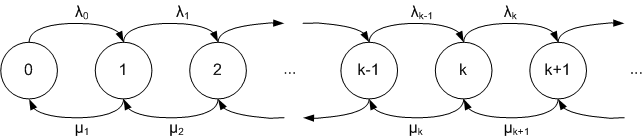
\includegraphics[scale=0.65]{images/BD-process.png}
\end{figure}

\noindent
The relationship between the birth and death rates and the state transition probabilities is given by:
\begin{align*}
    v_0 &= \lambda_0 \\
    v_i &= \lambda_i + \mu_i, \quad i > 0 \\
    P_{01} &= 1 \\
    P_{i, i + 1} &= \frac{\lambda_i}{\lambda_i + \mu_i}, \quad i > 0 \\
    P_{i, i - 1} &= \frac{\mu_i}{\lambda_i + \mu_i}, \quad i > 0
\end{align*}

\newpage
\noindent
Let $T_i$ denote the time, starting from state $i$, until the process enters state $i + 1$.
We can calculate the expected time $E(T_i)$ as follows:
\[ E(T_i) = \frac{1}{\lambda_i + \mu_i} + \frac{\mu_i}{\lambda_i + \mu_i}(E(T_{i - 1}) + E(T_i)) \]

\noindent
The first term represents the case where the next event is a birth, in which case we can simply take the exponentially distributed rate $\lambda_i + \mu_i$.
The second term represents the case where the next event is a death, in which case we must first get back to state $i$ before we can move to state $i + 1$.
We can also write the above equation as:
\[ E(T_i) = \frac{1}{\lambda_i} + \frac{\mu_i}{\lambda_i}E(T_{i - 1}), \quad i \geq 1 \]

\noindent
Starting with $E(T_0) = \frac{1}{\lambda_0}$, we can use the above formula to successively calculate $E(T_1)$, $E(T_2)$, and so on.
We can also use the sum $E(T_i) + E(T_{i + 1}) + ... + E(T_{j - 1})$ to calculate the expected time to move from state $i$ to state $j$.

\subsubsection{Limiting Probabilities}
Let $P_j$ denote the limiting probability that the process is in state $j$ at any time.
Instead of solving $\pi = \pi P$, we solve the balance equations:
\[ \text{outgoing flow of } P_j = \text{ incoming flow of } P_j \]

\noindent
For a birth-death process, the balance equations are given by:
\begin{align*}
    \lambda_0 P_0 &= \mu_1 P_1 \\
    (\lambda_n + \mu_n) P_n &= \mu_{n + 1}P_{n + 1} + \lambda_{n - 1}P_{n - 1}
\end{align*}

\noindent
By using $\displaystyle \sum_n P_n = 1$, we can find the following limiting probabilities:
\begin{align*}
    P_0 &= \frac{1}{\displaystyle 1 + \sum_{n = 1}^\infty \frac{\lambda_0 \lambda_1 \dots \lambda_{n - 1}}{\mu_1 \mu_2 \dots \mu_n}} \\
    P_n &= \frac{\lambda_0 \lambda_1 \dots \lambda_{n - 1}}{\displaystyle \mu_1 \mu_2 \dots \mu_n \left( 1 + \sum_{n = 1}^\infty \frac{\lambda_0 \lambda_1 \dots \lambda_{n - 1}}{\mu_1 \mu_2 \dots \mu_n} \right)}, \quad n \geq 1
\end{align*}

\noindent
In an irreducible continuous-time Markov chain with bounded rates, we have:
\[ P_j = \frac{\displaystyle \frac{\pi_j}{v_j}}{\displaystyle \sum_{i \in S} \frac{\pi_i}{v_i}}, \quad j \in S \]

\noindent
Furthermore, $\displaystyle E(T_j) = \frac{1}{v_j}$.

\newpage
\subsection{Queueing Theory}
Some fundamental concepts in queueing theory are:

\begin{itemize}
    \item $L$: The average number of customers in the system.
    \item $L_Q$: The average number of customers in the queue.
    \item $W$: The average time a customer spends in the system.
    \item $W_Q$: The average time a customer spends in the queue.
\end{itemize}

\noindent
These quantities are linked together through Little's law:
\[ L = \lambda_a W \]

\noindent
Where $\lambda_a$ is the average arrival rate of customers.
A different way to calculate $L$ is by using the following formula:
\begin{align*}
    L = \sum_{n = 0}^\infty n P_n && L_Q = \sum_{n = 1}^\infty (n - 1) P_n
\end{align*}

\noindent
Where $P_n$ is the limiting probability that the system contains $n$ customers.

\noindent
\\
For Poisson arrivals, the probability of the state as seen by an outside observer is the same as the probability of the state as seen by an arriving customer.
This is known as the \textbf{PASTA} property: Poisson Arrivals See Time Averages.

\subsubsection{Single-Server Queueing Systems}
Suppose that customers arrive at a single-server service station according to a Poisson process with rate $\lambda$.
That is, the time between two consecutive arrivals is exponentially distributed with mean $\frac{1}{\lambda}$.
The successive service times are also exponentially distributed with mean $\frac{1}{\mu}$.
This is called an $M/M/1$ queueing system.
The two $M$s refer to the fact that both the interarrival times and the service times are exponentially distributed (and thus memoryless), and the $1$ refers to the fact that there is only one server.

\noindent
\\
An important property of the $M/M/1$ queueing system is that the rate at which the process enters state $n$ equals the rate at which it leaves state $n$:
\begin{align*}
    \lambda P_0 &= \mu P_1 \\
    (\lambda + \mu)P_n &= \lambda P_{n - 1} + \mu P_{n + 1}
\end{align*}

\noindent
Using the fact that all $P_n$ must sum to $1$, we can calculate the limiting probabilities $P_n$ as follows:
\begin{align*}
    P_0 &= 1 - \frac{\lambda}{\mu} \\
    P_n &= \left( \frac{\lambda}{\mu} \right)^n P_0, \quad n \geq 1
\end{align*}

\noindent
Note that for these limiting probabilities to exist, $\frac{\lambda}{\mu} < 1$.

\newpage
\noindent
We can now calculate the fundamental concepts shown before as follows:
\begin{align*}
    L &= \frac{\lambda}{\mu - \lambda} \\
    L_Q &= \frac{\lambda^2}{\mu(\mu - \lambda)} \\
    W &= \frac{1}{\mu - \lambda} \\
    W_Q &= \frac{\lambda}{\mu(\mu - \lambda)}
\end{align*}

\noindent
Furthermore, the amount of time a customer spends in the system, $W^*$, is an exponential random variable with rate $\mu - \lambda$.

\subsubsection{Single-Server Queueing Systems with Finite Capacity}
In the previous model, we assumed that there was no limit on the number of customers that could be in the system at the same time.
However, in reality there is always a finite system capacity $N$, in the sense that there can be no more than $N$ customers in the system at any time.
By this, we mean that if an arriving customer finds that there are already $N$ customers present, then they do not enter the system.
The rate-equality equations for an $M/M/1$ queueing system with finite capacity are given by:
\begin{align*}
    \lambda P_0 &= \mu P_1 \\
    (\lambda + \mu)P_n &= \lambda P_{n - 1} + \mu P_{n + 1} \\
    \mu P_N &= \lambda P_{N - 1}
\end{align*}

\noindent
Which can be reduced to the following equation:
\[ P_n = \frac{\left( \frac{\lambda}{\mu} \right)^n \left( 1 - \frac{\lambda}{\mu} \right)}{1 - \left( \frac{\lambda}{\mu} \right)^{N + 1}}, \quad n = 0, 1, ... , N \]

\noindent
Note that in this case, there is no need to impose the condition that $\frac{\lambda}{\mu} < 1$, as the queue size is by definition limited to $N$.

\noindent
\\
We say that a queueing system alternates between \textbf{idle} periods when there are no customers in the system and \textbf{busy} periods in which there is at least one customer in the system.
Let $L_N$ denote the number of lost customers in a busy period of a finite-capacity $M/M/1$ queueing system.
We say that a customer is lost if they arrive at the system and find that there are already $N$ customers present.
The expected number of lost customers in a busy period is given by:
\begin{align*}
    E(L_N) &= \left( \frac{\lambda}{\mu} \right)^N \\
    Var(L_N) &= \left( \frac{\lambda}{\mu} \right)^N + 2 \sum_{j = N + 1}^{2N - 1} \left( \frac{\lambda}{\mu} \right)^j + \left( \frac{\lambda}{\mu} \right)^{2N}
\end{align*}

%
% Chapter 5 - Multi-Armed Bandits
%
\newpage
\section{Multi-Armed Bandits}
Imagine that we want to go to a restaurant every night, and we have a choice between restaurant $A$, $B$, and $C$.
At the end of each night, we receive a reward based on how good the food was.
This reward is sampled from a distribution that is specific to each restaurant (i.e. we will not always get the same reward at the same restaurant).
The goal is to maximize the total reward we receive over a certain period of time, while not knowing the reward distributions of the restaurants a priori.
This problem is an example of the \textbf{multi-armed bandit problem}.

\noindent
\\
Let $A = \{ 1, 2, ... , k \}$ be a finite set of actions (also called arms).
At each time $t = 1, 2, ...$, the player selects an action $a_t \in A$, and receives a reward $X_t \sim P_{A_t}$.
The goal is to maximize the total reward $\sum_t X_t$, while not knowing the reward distributions $P_1, P_2, ... , P_k$ and the stopping time a priori.
An important distinction between Markov chains, MDPs, and multi-armed bandits is that a multi-armed bandit problem does not have a state space.

\subsection{Evaluating MAB Algorithms}
We can \textit{empirically} evaluate the performance of multiple MAB algorithms by comparing either the total reward $\sum_t^T X_t$ or the average reward $\displaystyle \frac{\sum_t^T X_t}{T}$.

\noindent
\\
We can \textit{theoretically} evaluate the performance of MAB algorithms by performing a \textbf{regret analysis}.
The \textbf{regret} of a policy $\pi$ is the difference in rewards that we expect to collect in $n$ steps if we always pull the optimal arm $a^*$, compared to what we expect to get when pulling arms according to the policy $\pi$:
\[ R_n(\pi) = n\mu_{a^*} - E\left( \sum_{t = 1}^n X_t \right) \]

\noindent
What makes MAB problems difficult is that the player must balance the exploration of new arms with the exploitation of arms that have already shown to be good.
Some arms that have a low reward in the beginning may have a high reward in the long run, and vice versa.

\subsection{MAB Algorithms}
\subsubsection{Explore-Then-Commit (ETC)}
The \textbf{Explore-Then-Commit} algorithm is a simple MAB algorithm that first explores each arm $m$ times, and then commits to the arm with the highest average reward.
Note that the mean reward of the selected arm will still be updated after the exploration phase.
This is usually done by keeping track of the sum of observed rewards and the number of times the arm has been pulled:
\[ \hat{\mu}_t = \frac{\displaystyle\sum_{i = 1}^t X_i}{t} \]

\noindent
The problem with this approach is that the sum of rewards may overflow if the rewards are large, or if the arm is pulled many times.
A better approach is to incrementally update the mean using the current mean:
\[ \hat{\mu}_t = \hat{\mu}_{t - 1} + \frac{X_t - \hat{\mu}_{t - 1}}{t} \]

\newpage
\noindent
Returning back to the ETC algorithm, performing a regret analysis shows that the regret of the ETC algorithm is bounded by:
\[ R_n \leq m \sum_{i = 1}^k \Delta_i + (n - mk) \sum_{i = 1}^k \Delta_i e^{\displaystyle-\frac{m\Delta_i^2}{4}} \]

\noindent
Where $\Delta_i = \mu_{a^*} - \mu_i$ is the suboptimality gap of arm $i$, $m$ is the number of exploration rounds, and $n - mk$ is the number of exploitation rounds.
The left part of the sum represents the guaranteed regret from the exploration phase, while the right part represents an upper bound on the regret from the exploitation phase.

\subsubsection{$\epsilon$-Greedy}
The \textbf{$\epsilon$-Greedy} algorithm is another simple MAB algorithm that selects the best arm with probability $1 - \epsilon$, and selects a random arm with probability $\epsilon$.
For $\epsilon$-Greedy to converge to the optimal arm, the following conditions must hold:

\begin{enumerate}
    \item \textbf{Infinite Exploration:} $\epsilon_t > 0$ for all finite $t$.
    \item \textbf{Decaying Exploration:} $\displaystyle \lim_{t \rightarrow \infty} \epsilon_t = 0$ (e.g. $\epsilon_t = \frac{1}{t}$).
\end{enumerate}

\noindent
Note that in practice, $\epsilon$ is often simply set to a small constant value.

\noindent
\\
The exploration mechanism of $\epsilon$-Greedy is \textbf{uninformed}: it chooses an arm uniformly at random, with no bias towards either close-to-best or under-explored arms.

\noindent
\\
A possible way to add bias to the exploration is to use \textbf{optimistic value initialization}.
This means that we initialize the mean reward of each arm to an estimate of the upper bound of the mean reward, and pretend that we have already observed a number of rewards $N \geq 1$ from each arm.
Since the true mean reward is likely lower than the initial estimate, the algorithm will end up exploring under-explored arms more often.

\subsubsection{Upper Confidence Bounds (UCB1)}
If we are uncertain about the mean reward of an arm, we should be optimistic:
If we get a high reward, we will be happy.
If we get a low reward, we will have learned something new:

\begin{figure}[h]
    \centering
    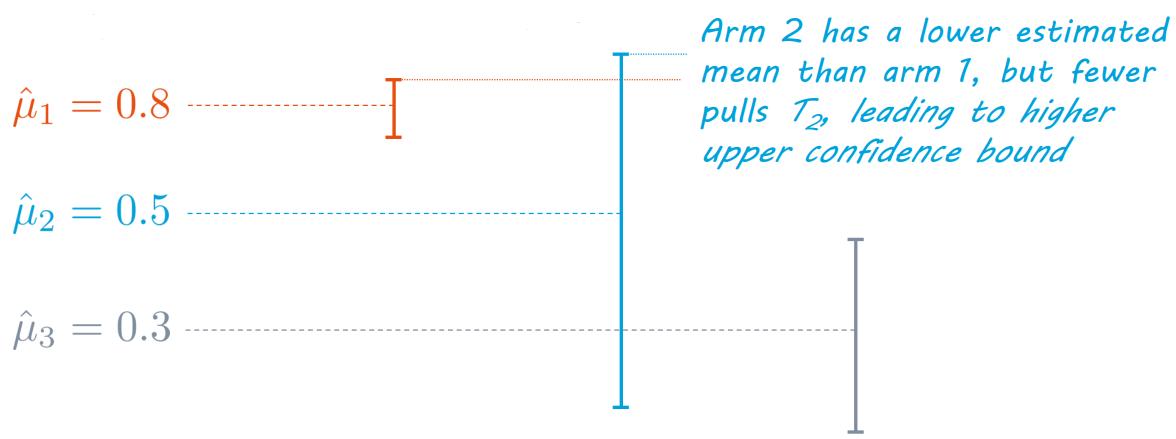
\includegraphics[scale=0.55]{images/UCB.PNG}
\end{figure}

\newpage
\noindent
We can use the following inequality to calculate an \textbf{upper confidence bound} on the mean reward of an arm:
\[ P\left( \hat{\mu} + \sqrt{\frac{2 \log(\frac{1}{\delta})}{n}} \leq \mu^* \right) \leq \delta \]

\noindent
The probability that the term $\displaystyle \hat{\mu} + \sqrt{\frac{2 \log(\frac{1}{\delta})}{n}}$ underestimates the true mean $\mu^*$ is bounded by $\delta \in (0, 1)$.
This is used by the \textbf{Upper Confidence Bounds Algorithm} as follows:
\[ A_t \leftarrow \arg \max_a \begin{cases}
    \infty & \text{if } T_a = 0 \\
    \displaystyle \hat{\mu}_a + \sqrt{\frac{2 \log(\frac{1}{\delta})}{T_a}} & \text{otherwise}
\end{cases} \]

\noindent
Here the $\hat{\mu}_a$ term acts as the exploitation term, while the rest of the formula acts as the exploration term.
If $\delta$ is constant, this is a function that can only decrease over time.
This means that we may not have infinite exploration in the limit, which is a requirement for an algorithm to converge to the optimal arm.
A solution to this is to set $\delta$ in a different way, most famously as done in the \textbf{UCB1} algorithm:
\[ \hat{\mu}_a + C \sqrt{\frac{\log(t)}{T_a}} \]

\noindent
Replacing $\frac{1}{\delta}$ by $t$ causes the upper bound of arms that are not pulled to gradually increase over time, guaranteeing infinite exploration in the limit.
Note that the $2$ was also replaced by a hyperparameter $C$, often called the \textbf{exploration parameter}.

\subsubsection{Stochastic Gradient Bandit}
All the previous algorithms estimate the mean reward of each arm and use this estimate to select the best arm.
An alternative approach is to learn an arbitrary value for each arm, and use their relative ordering to select the best arm.
Such an arbitrary value is called a \textbf{preference}.
A \textbf{policy} is a function that uses the preferences to select an arm, a common example being the \textbf{softmax policy}:
\[ \pi_t(a) = P(A_t = a) = \frac{e^{z_t(a)}}{\displaystyle \sum_{b = 1}^k e^{z_t(b)}} \]

\noindent
Here $\pi_t(a)$ is the probability of selecting arm $a$ at time $t$, and $z_t(a)$ is the preference of arm $a$ at time $t$, where $k$ is the number of arms.

\noindent
\\
The question now becomes how to learn these preference values.
For this, we can use \textbf{Stochastic Gradient Ascent}.
Gradient ascent is a method to find the maximum of a function $f_\theta(x)$, given a dataset $D$ with lots of example inputs $x$.
$\theta$ is optimized by iteratively updating it in the direction of the gradient, computed over the dataset $D$.
Stochastic gradient ascent is a variant of gradient ascent that only uses a small subset of the dataset to compute the gradient.

\newpage
\noindent
The \textbf{Stochastic Gradient Bandit} algorithm uses stochastic gradient ascent to learn the preferences of each arm.
The algorithm works as follows:

\begin{enumerate}
    \item Select an arm $A_t$ according to the softmax policy $\pi_t$: $A_t \sim \pi_t$.
    \item Observe the reward $X_t \sim P_{A_t}$.
    \item Update the preference of the selected arm using stochastic gradient ascent:
    \[ z_{t + 1}(A_t) \leftarrow z_t(A_t) + \alpha X_t (1 - \pi_t(A_t)) \]
    Where $\alpha$ is the learning rate. The intuition is to push the arm preference up or down proportional to the magnitude and sign of the reward $X_t$.
    This magnitude is further increased if the arm was selected with a low probability $1 - \pi_t(A_t)$, or decreased if the arm was selected with a high probability $\pi_t(A_t)$.
    \item Update the preferences of the other arms:
    \[ z_{t + 1}(a) \leftarrow z_t(a) - \alpha X_t \pi_t(a) \]
    For all $a \neq A_t$.
\end{enumerate}

\subsection{Contextual Bandits}
The \textbf{Contextual Multi-Armed Bandit} problem is an extension of the regular multi-armed bandit problem.
Going back to the restaurant example, we may have additional information about the restaurants, such as the type of food, the price, reviews, etc.
This additional information is called the \textbf{context} or \textbf{features} of the arms.
Context can either be per-arm or global.
An example of global context would be what you ate yesterday, or the current weather or season.
Note that we must always have at least one per-arm feature.

\noindent
\\
Let $A = \{ 1, 2, ... , k \}$ be a set of actions in a CMAB problem.
Note that, now that we have context, it becomes possible to solve multi-armed bandit problems with a continuous or variable-size action space.
Let $C \subseteq \mathbb{R}^d$ be the $d$-dimensional context space, and let $P$ be the reward distribution of the arms, given context $\phi \in C$.
Note that we are no longer explicitly enumerating different probability distributions per arm.
Instead, the context fully determines the reward distribution.
If necessary, we could still encode the arm identity into the context vector.
At every time $t$, we observe context vectors $\{ \phi_t^1 \in C, ... , \phi_t^k \in C \}$ for all $k$ arms, select an action $A_t \in A$, and receive a reward $X_t \sim P(x | \phi_t^{A_t})$.

\noindent
\\
Global features are shared among all arms within the same time step.
To encode this, we can simply append a copy of the global feature vector to each arm's per-arm feature vector:

\begin{figure}[h!]
    \centering
    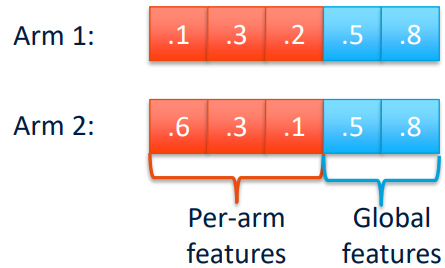
\includegraphics[scale=0.6]{images/featurevectors.PNG}
\end{figure}

\newpage
\noindent
We can also apply all the standard practices of machine learning to the feature vectors, for example:

\begin{itemize}
    \item We can select more interesting features, while removing uninformative features (remember that the end goal of any CMAB problem is to maximize the reward).
    \item Many algorithms behave better with binary features or numeric features normalized to either $[0, 1]$ or $[-1, 1]$.
    \item Deep learning is a good idea when the feature space is large or complex.
\end{itemize}

\subsubsection{Linear Contextual Bandits}
To keep things simple, we will assume that the true mean of the reward distribution is a linear function of the context (and thus we can predict rewards $X_t$ as a linear function of the features $\phi_t^{A_t}$):
\begin{align*} 
    \mu^*(\phi) = \phi^T \theta^* && X_t \approx \hat{\theta}^T \phi_t^{A_t}
\end{align*}

\noindent
Where $\theta^*$ is the optimal parameter vector that we want to learn.
The easiest way to learn $\hat{\theta} \approx \theta^*$ is to use \textbf{linear regression}.
When performing linear regression we assume that every feature vector has a bias term $x_0 = 1$.
The most classic example of linear regression is fitting a line to a set of points.
Since not every point will lie exactly on the line, we can minimize the sum of squared errors to find the best-fitting line:
\[ \hat{\theta} = \min_\theta \frac{1}{2m} \sum_{i = 1}^m (y^{(i)} - \theta^T \phi^{(i)})^2 \]

\noindent
A problem with linear regression is that it may not behave well when features are strongly correlated with each other.
The solution to this is to use \textbf{ridge regression}, which adds a regularization term to the loss function:
\[ \hat{\theta} = \min_\theta \left( \left( \frac{1}{2m} \sum_{i = 1}^m (y^{(i)} - \theta^T \phi^{(i)})^2 \right) + \lambda \left\lVert \theta \right\rVert_2^2 \right) \]

\noindent
Ridge regression can be computed incrementally as:
\[ \hat{\theta}_t = V_t^{-1}b_t \]

\noindent
Where $V_t$ is a $d \times d$ matrix that accumulates the sum of the per-sample feature values multiplied with each other, and $b_t$ is a $d$-dimensional vector that accumulates greater values for entries corresponding to features that are correlated with high rewards.
Computing ridge regression incrementally has some potential issues, such as matrix inversion being computationally expensive, and the entries of $V_t$ and $b_t$ possibly growing forever.
To solve this, we can also use \textbf{stochastic gradient descent} to learn the optimal parameter vector $\theta$:
\[ \hat{\theta}_{t + 1} = \left( 1 - \alpha \frac{\lambda}{m} \right) \hat{\theta}_t - \alpha \left( \frac{1}{m} \sum_{i = 1}^m \left( \hat{\theta}_t^T \phi^{(i)} - y^{(i)} \right) \phi^{(i)} \right) \]

\noindent
Notice the regularization term $\left( 1 - \alpha \frac{\lambda}{m} \right)$.
In CMABs, $m$ is usually equal to 1: the feature vector $\phi^{(i)}$ and the reward $y^{(i)}$ for the arm we ended up selecting:
\[ \hat{\theta}_{t + 1} = (1 - \alpha \lambda) \hat{\theta}_t - \alpha \left( \left( \hat{\theta}_t^T \phi_t^{A_t} - X_t \right) \phi_t^{A_t} \right) \]

\newpage
\noindent
A final note on linear CMABs is that global features are useless in a linear model.
Since global features are the same for all arms, they will not affect the relative ordering of the arms, instead only adding a flat error term to the reward prediction.
A solution to this is to either construct new features that are a combination of the global and per-arm features, or to use a non-linear model.
Additionally, if the number of arms is fixed, we can train a separate linear model for each arm, but this becomes troublesome if new arms are introduced later on.

\subsubsection{Linear CMAB Algorithms}
We will now try to convert the regular MAB algorithms to work with (linear) contextual bandits, starting with \textbf{Explore-Then-Commit (ETC)}:

\begin{enumerate}
    \item Explore each arm $m$ times, updating the means $\rightarrow$\\ \-\, Instead of updating the means, update the linear model.
    \item Permanently commit to the best-performing arm $\rightarrow$\\ \-\, Commit by always playing greedily according to the linear model.
\end{enumerate}

\noindent
The problem with ETC in linear CMABs is that the arm identity might not be relevant at all.
Furthermore, the number of arms may be dynamic.
This leads to ETC never being used in practice for linear CMABs.

\noindent
\\
Next, we will convert the \textbf{$\epsilon$-Greedy} algorithm to work with linear CMABs:

\begin{enumerate}
    \item Track empirical means $\hat{\mu}_i$ $\rightarrow$\\ \-\, Instead of tracking the means, update the linear model.
    \item Select an arm uniformly at random with probability $\epsilon$.
    \item Select an arm greedily with probability $1 - \epsilon$ $\rightarrow$\\ \-\, Select an arm greedily according to the linear model.
\end{enumerate}

\noindent
Next up is the \textbf{Upper Confidence Bounds (UCB1)} algorithm, which is a bit more complicated to convert to linear CMABs.
Upper confidence bounds are calculated using the per-arm count $T_a$, which is meaningless in linear CMABs.
This means that we need to find another way to compute meaningful bounds.
The \textbf{LinUCB} algorithm comes up with the following bounds:
\[ \left\lvert \hat{\theta}^T \phi_t^{A_t} - E\left( X_t | \phi_t^{A_t} \right) \right\rvert \leq \left( 1 + \sqrt{\frac{\log \left( \frac{2}{\delta} \right)}{2}} \right) \sqrt{\phi_t^{A_t T} V_t^{-1} \phi_t^{A_t}}  \]

\noindent
With probability $1 - \delta$, the true mean reward $X_t$ is within the bounds of the predicted mean reward $\hat{\theta}^T \phi_t^{A_t}$.
The left side of the inequality is the difference between the predicted and true mean reward, while the right side can be seen as an additive exploration term.
This term gets added to the predicted mean reward, and the arm with the highest final value is selected.
Note that these bounds only apply to $\hat{\theta}$ computed using the analytical solution to ridge regression (i.e. not stochastic gradient descent).

\newpage
\noindent
Lastly, we have the \textbf{Stochastic Gradient Bandit} algorithm, which can be converted to linear CMABs as follows:

\begin{enumerate}
    \item Define a softmax policy $\displaystyle \pi_t(a) = \frac{e^{z_t(a)}}{\sum_{b = 1}^k e^{z_t(b)}}$ $\rightarrow$\\ \-\, We can make $z_t(a) = \theta^T \phi_t^a$ a linear function instead of a scalar.
    \item Take stochastic gradient ascent steps to maximize the reward $\rightarrow$\\ \-\, Update the linear model using stochastic gradient descent:
    \[ \theta \leftarrow \theta + \alpha X_t \left( \phi_t^{A_t} - \frac{1}{k} \sum_{i = 1}^k \pi_t(i)\phi_t^i \right) \]
\end{enumerate}

\subsection{Pure Exploration}
In the previous sections, we have focused on algorithms that balance exploration and exploitation.
However, in some cases, we may only be interested in exploration.
What if we only care to optimise the outcome at a specific final time step?
This would mean that time steps $1, 2, ... , n$ are purely used for exploration, and the final time step $n + 1$ is used for exploitation.
This is called a \textbf{pure exploration} setting.

\noindent
\\
This is essentially just a standard MAB problem, but with a different evaluation criterion.
Instead of the cumulative regret, we only care about the simple regret at the final time step:
\[ R_n^{\text{SIMPLE}}(\pi) = \left( \max_{1 \leq a \leq k} \mu_a \right) - E_{A_t \sim \pi}(X_{n + 1}) \]

\noindent
Note that just because the problem is called pure exploration, it does not mean that we do not need any preference for high-performing arms.
Focusing more on high-performing arms will allow us to rank them more accurately.

\subsubsection{Sequential Halving}
The \textbf{Sequential Halving} algorithm is a simple pure exploration algorithm that assumes that the fixed step budget $n$ is known in advance.
The algorithm works as follows:

\begin{enumerate}
    \item Divide the budget over $L = \left\lceil \log_2(k) \right\rceil$ phases: $\left\lfloor \frac{n}{L} \right\rfloor$ steps per phase.
    \item For each phase, pull each arm equally many times. Keep track of the mean reward for each arm:
    \[ T_{l \in L} = \left\lfloor \frac{n}{L |A|} \right\rfloor \]
    Note that, for mathematical reasons, we should only estimate the mean reward using data collected in the current phase.
    \item After each phase, discard the worst-performing half of the arms.
\end{enumerate}

\noindent
At time $n + 1$, $A$ will only contain the best-performing arm.

\end{document}
